\section{Data and Preprocessing}
\subsection{Data-set}
The Fashion-MNIST is a data-set of Zalando's article images—consisting of a training set of 60,000 samples and 10,000 test samples. The data-set used here is a small portion of the original data-set, 10,000 training and 5,000 test samples. Each sample is a 28x28 pixels gray-scale image with a label indicating the type of clothing item associated with each. 
\newline

\begin{figure}[ht]
\centering
\includegraphics[scale=0.45]reports/figures_for_report/samples_from_classes.png}
\captionsetup{justification=centering,margin=2cm}
\caption{One sample from each class (reconstructing images from pixels)}
\end{figure}
\subsection{Naming Conventions}
The exploration of samples within each class gave rise to more appropriate names. Class 0 became T-shirt etc. Below is our naming conventions, which we will use throughout the report for better readability.  \\
\begin{table}[!ht]
  \footnotesize
  \centering
\begin{tabular}{ c c c c c }
 \toprule
 \textbf{0} & \textbf{1} & \textbf{2} & \textbf{3} & \textbf{4} \\ 
 \midrule 
 T-shirt & Pants & Sweatshirt & Dress & Shirt \\ 
 \bottomrule
\end{tabular} \\[0.2cm]
\captionsetup{justification=centering,margin=2cm}
\caption{Mapping from class-labels to clothing type}
\label{features}
\end{table}


\subsection{Data Cleaning}
The data-set provided was already in a cleaned state, which was verified by checking for missing values, and checking that the pixel values were no greater than 255 and no smaller than 0. 

\subsection{Preprocessing}
The pixels were in the range $[0, 255]$. This range was normalized to $[0, 1]$ by dividing each pixel by 255. This was done primarily to improve training time. % not sure if we need this tbh but it was recommended online see below

% 1 of many sources for this ^ https://machinelearningmastery.com/how-to-manually-scale-image-pixel-data-for-deep-learning/ %
\subsection{Class Distribution}
Whether or not a machine learning model can learn to predict classes well depends to a high degree on how those classes are distributed within our training and training data-set. Both our data-sets are extremely balanced, with the test being fully balanced ($1000$ of each class). This is illustrated on the plots below

\begin{figure}[ht]
\centering
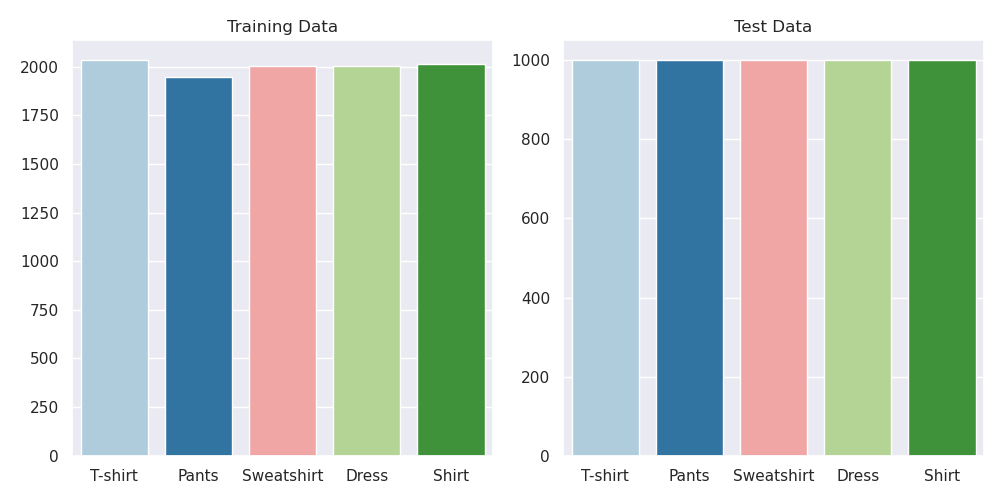
\includegraphics[scale=0.45]{figures/class_distribution.png}
\captionsetup{justification=centering,margin=2cm}
\caption{Distribution of clothing items in our training and test data-set}
\end{figure}

